% %%%%%%%%%%%%%%%%%%%%%%%%%%%%%%%%%%%%%%%%%%%%%%%%%%%%%%%%%%%%%%%%%%%%%
% %% State-of-the-Art %%
% Hardware Accelerators
% %%%%%%%%%%%%%%%%%%%%%%%%%%%%%%%%%%%%%%%%%%%%%%%%%%%%%%%%%%%%%%%%%%%%%

\section{Hardware Accelerators for Sparse Matrices and Vectors}
\label{sec:soa:hw_accelerators}

\lettrine{I}{n} this section, we describe the recent (2015-2025) hardware accelerators for sparse \acrshort{mm} and \acrshort{mv}, targeting mainly \acrshort{asic}-type implementation.
We note there are many \acrshort{fpga}-based accelerators, however, to limit the scope we do not focus on these and only include those which can be classified along the \acrshort{asic}-type accelerators.
We try to use consistent notation, for example in the color code in the architecture figures.
Particularly, all kinds of compute units are represented in \textit{red}, control units in \textit{orange}, all kinds of data transfer units in \textit{yellow}, caches in \textit{blue}, and all kinds of memories in \textit{green}.
We include our work, the \acrlong{spdc} accelerator~[\ref{publ:SpDC}], which we describe in subsequent chapters, as we published initial results in 2024.
Before going into detailed overviews of specific accelerators, in Table~\ref{tab:soa:classificationOverview} we present a criteria-based classification of the designs which were studied.

A first criterion to classify the accelerators is between \textit{standalone} accelerators that address the full kernel without the assist of a processor (\ex OuterSPACE~\cite{Pal2018_OuterSPACE}) and ones that address only a part of the kernel and need a processor to manage the computation (\ex PHI~\cite{Mukkara2019_PHI}).
Most of the \textit{standalone} accelerators are directly connected to the main memory and internally manage their internal memories.
Accelerators can also intervene at different levels of the memory hierarchy, giving a second classification criterion.
Certain accelerators intervene near the processors (\ex ASA~\cite{Zhang2022_ASA}), near the cache (\ex PHI), or near the main memory (\ex SPiDRE~\cite{Barredo2019_SPiDRE}).

Each accelerator is optimized for one or several specific algorithms (\acrshort{ip}, \acrshort{op} or \acrshort{gust}), our third criterion.
For example, some accelerators (\ex PHI) address the \gls{reduction} problem and are adapted to \acrshort{op} algorithms but \glspl{reduction} are also required with \acrshort{gust} and highly-tiled algorithms.
ExTensor~\cite{Hegde2019_ExTensor} is a general purpose accelerator that is demonstrated for a highly-tiled \acrshort{op} but also makes major contributions for \acrshort{ip}.

From a memory perspective, the two main problems are \gls{gather} and \gls{scatter}, our fourth criterion.
Certain accelerators offer solutions for one, the other or both.
For example, some accelerators (\ex OuterSPACE) are specialized for an \acrshort{op} algorithm but optimize both \gls{gather} and \gls{scatter}.
Finally, accelerators may be optimized for sparse \acrshort{mm}, \acrshort{mv} or both, our final criterion.

After this first comparison, in Sections~\ref{sec:soa:outerspace} to~\ref{sec:soa:phi} we present in detail three \textit{standalone} accelerators (\eg OuterSPACE, ExTensor and Gamma) and one \textit{processor-assist} accelerator (\eg PHI), which cover several types of architectures and algorithms.
In Section~\ref{sec:soa:other_accel}, we give bief descriptions on other accelerators from Table~\ref{tab:soa:classificationOverview}.

{
    \DefTblrTemplate{caption-sep}{default}{~--\enskip}
    \NewTblrTheme{fancy}{
        \SetTblrStyle{caption-tag}{font=\bfseries}
        \SetTblrStyle{caption-sep}{font=\bfseries}
    }
    \def\ck{\ding{51}}
    \def\sa{\ding{86}\textsuperscript{1}}
    \def\sb{\ding{86}\textsuperscript{2}}
    \def\sc{\ding{86}\textsuperscript{3}}
    \def\sd{\ding{86}\textsuperscript{4}}
    \begin{longtblr}[
            theme = fancy,
            caption = {Algorithmic and Architectural Classification of Existing Accelerators},
            label = {tab:soa:classificationOverview},
        ]{
            width = {\linewidth},
            colspec = {X[3,c] X[1,c] *{12}{X[1,c]}}, % rowspec
            rows = {m, font=\footnotesize},
            colsep = {1pt},
            rowhead = 2,
            rowfoot = 4,
            row{1-W} = {rowsep=2pt, black!2},
            row{1-2} = {c, font=\bfseries\footnotesize, black!5},
            cell{2}{3-7,13-14} = {font=\bfseries\itshape\footnotesize},
            row{W-Z} = {l, font=\itshape\footnotesize, rowsep=-2pt},
            row{W} = {abovesep=2pt},
            row{Z} = {belowsep=2pt},
            cell{1}{1,2} = {r=2}{valign=f},
            cell{2}{3-12} = {cmd=\rotatebox{90}},
            cell{1}{3,11,13} = {c=2}{},
            cell{1}{5,8} = {c=3}{},
            cell{W-Z}{1} = {c=14}{},
            hspan = {minimal},
            % hlines, vlines,
            % rulesep = {-1pt},
            hline{1,V} = {2pt}, % Z for last
            hline{3} = {1pt},
            hline{Z} = {1pt, dashed},
            vline{2,3,5,8,11,13} = {1-V}{0.5pt},
        }
        %
        Name & Year & Autonomy & & {Position in \\ Memory Hierarchy} & & & {Most Adapted \\ Algorithm(s)} & & & {Hardware \\ Support for} & & {Sparse \\ Kernels \\ Addressed} & \\
        & & Standalone & Processor-Assist & Near Processors & Near Caches & Near Main Memory & \acrlong{ip} & \acrlong{op} & \acrlong{gust} & \Gls{gather} & \Gls{scatter} & \acrshort{mv} & \acrshort{mm} \\
        %
        Coup~\cite{Zhang2015_Coup}                    & 2015 &     & \ck &     & \ck &     &     & \ck &     &     & \ck & \ck & \sc \\
        EIE~\cite{Han2016_EIE}                        & 2016 & \ck &     &     &     & \sa &     & \ck &     & \ck & \ck & \ck &     \\
        OuterSPACE~\cite{Pal2018_OuterSPACE}          & 2018 & \ck &     &     &     & \sa &     & \ck &     & \ck & \ck & \ck & \ck \\
        GraphR~\cite{Song2018_GraphR}                 & 2018 & \ck &     &     &     & \sa &     & \ck &     & \ck & \ck & \ck &     \\
        SDE~\cite{Hosseinabady2019_SDE}               & 2019 & \ck &     &     &     & \sa & \ck &     & \sc & \ck & \sb & \ck & \sc \\
        ExTensor~\cite{Hegde2019_ExTensor}            & 2019 & \ck &     &     &     & \sa & \ck & \sb &     & \ck & \sb & \sc & \ck \\
        PHI~\cite{Mukkara2019_PHI}                    & 2019 &     & \ck &     & \ck &     &     & \ck & \sc &     & \ck & \ck & \sc \\
        SPiDRE~\cite{Barredo2019_SPiDRE}              & 2019 &     & \ck &     &     & \ck & \ck &     &     & \ck &     & \ck & \sc \\
        ITS~\cite{Sadi2019_ITS}                       & 2019 & \ck &     &     &     & \sa &     & \ck &     & \ck & \ck & \ck &     \\
        SPU~\cite{Dadu2019_SPU}                       & 2019 & \ck &     &     &     & \sa & \ck & \ck &     & \ck & \ck & \ck &     \\
        Tensaurus~\cite{Srivastava2020_Tensaurus}     & 2020 & \ck &     &     &     & \sa & \sc & \sb &     & \ck & \ck & \ck & \ck \\
        MatRaptor~\cite{Srivastava2020_MatRaptor}     & 2020 & \ck &     &     &     & \sa &     &     & \ck & \ck & \ck &     & \ck \\
        SpArch~\cite{Zhekai2020_SpArch}               & 2020 & \ck &     &     &     & \sa &     & \ck &     & \ck & \ck &     & \ck \\
        Alrescha~\cite{Asgari2020_Alrescha}           & 2020 & \ck &     &     &     & \sa & \ck &     &     & \ck & \ck & \ck &     \\
        SIGMA~\cite{Qin2020_SIGMA}                    & 2020 & \ck &     &     &     & \sa & \ck &     &     & \ck & \ck &     & \ck \\
        SpaceA~\cite{Xie2021_SpaceA}                  & 2021 & \ck &     &     &     & \ck & \ck &     &     & \ck & \ck & \ck &     \\
        Gamma~\cite{Zhang2021_Gamma}                  & 2021 & \ck &     &     &     & \sa &     &     & \ck & \ck & \ck &     & \ck \\
        SPAGHETTI~\cite{Hojabr2021_SPAGHETTI}         & 2021 & \ck &     &     &     & \sa &     & \ck &     & \ck & \ck &     & \ck \\
        InnerSP~\cite{Baek2021_InnerSP}               & 2021 & \ck &     &     &     & \sa &     &     & \ck & \ck & \ck &     & \ck \\
        CoSPARSE~\cite{Feng2021_CoSPARSE}             & 2021 & \ck &     &     &     & \sa & \ck & \ck &     & \ck & \ck & \ck &     \\
        SortCache~\cite{Srikanth2021_SortCache}       & 2021 &     & \ck &     & \ck &     &     & \ck & \sc &     & \ck & \sc & \ck \\
        Sextans~\cite{Song2022_Sextans}               & 2022 & \ck &     &     &     & \sa &     & \ck &     & \ck & \ck &     & \ck \\
        ASA~\cite{Zhang2022_ASA}                      & 2022 &     & \ck & \ck &     &     &     & \sc & \ck &     & \ck & \sc & \ck \\
        Spada~\cite{Li2023_Spada}                     & 2023 & \ck &     &     &     & \sa &     &     & \sd & \ck & \ck &     & \ck \\
        Flexagon~\cite{Munoz-Martinez2023_Flexagon}   & 2023 & \ck &     &     &     & \sa & \ck & \ck & \ck & \ck & \ck &     & \ck \\
        MOSCON~\cite{Noble2023_MOSCON}                & 2023 & \ck &     &     &     & \sa &     & \ck &     & \ck & \ck &     & \ck \\
        GSCSp~\cite{Li2023_GSCSp}                     & 2023 & \ck &     &     &     & \sa &     &     & \ck & \ck & \ck &     & \ck \\
        SDMA~\cite{Gao2023_SDMA}                      & 2023 & \ck &     &     &     & \sa &     &     & \sd & \ck & \ck &     & \ck \\
        SSSR~\cite{Scheffler2023_SSSR}                & 2023 &     & \ck & \ck &     &     & \ck &     &     & \ck &     & \ck & \sc \\
        Funnel~\cite{Ma2024_Funnel}                   & 2024 & \ck &     &     &     & \sa & \ck &     & \ck & \ck & \ck &     & \ck \\
        GAS~\cite{Zhang2024_GAS}                      & 2024 & \ck &     &     &     & \ck &     & \ck &     &     & \ck & \ck & \ck \\
        ACES~\cite{Lu2024_ACES}                       & 2024 & \ck &     &     &     & \sa &     &     & \ck & \ck & \ck &     & \ck \\
        FullSparse~\cite{Yu2024_FullSparse}           & 2024 & \ck &     &     &     & \sa &     & \ck &     & \ck & \ck &     & \ck \\
        Sparm~\cite{Luo2024_Sparm}                    & 2024 & \ck &     &     &     & \sa & \ck & \ck & \ck & \ck & \ck &     & \ck \\
        \textbf{SpDCache}~[\ref{publ:SpDC}]           & 2024 &     & \ck &     & \ck &     &     & \ck & \sc &     & \ck & \ck & \sc \\
        SPADES~\cite{Huang2024_SPADES}                & 2024 & \ck &     &     &     & \sa & \sc & \sc & \sc & \ck &     & \ck & \sc \\
        DySpMM~\cite{Wang2024_DySpMM}                 & 2024 & \ck &     &     &     & \sa & \ck &     &     & \ck & \ck &     & \ck \\
        Vesper~\cite{Jin2024_Vesper}                  & 2024 & \ck &     &     &     & \sa & \ck & \ck & \ck & \ck & \ck & \ck & \ck \\
        Mentor~\cite{Lu2024_Mentor}                   & 2024 & \ck &     &     &     & \sa &     &     & \ck & \ck & \ck &     & \ck \\
        IOPS~\cite{Sun2025_IOPS}                      & 2025 & \ck &     &     &     & \sa & \ck & \ck &     & \ck & \ck &     & \ck \\
        Leda~\cite{Yi2025_Leda}                       & 2025 & \ck &     &     &     & \sa &     & \ck &     & \ck & \ck &     & \ck \\
        DMSA~\cite{Nagahara2025_DMSA}                 & 2025 & \ck &     &     &     & \sa &     &     & \sd & \ck & \ck &     & \ck \\
        C\textsuperscript{3}ache~\cite{li2025_C3ache} & 2025 &     & \ck &     & \ck &     &     & \sd & \sd & \ck & \ck &     & \ck \\
        ScanNow~\cite{Ma2025_ScanNow}                 & 2025 & \ck &     &     &     & \sa &     &     & \sd & \ck & \ck &     & \ck \\
        %
        \sa \; Most standalone accelerators connect directly to main memory. \\
        \sb \; Not main contribution but addressed in the article. \\
        \sc \; Could be adapted but not discussed in the article. \\
        \sd \; New complex algorithm inspired by.
    \end{longtblr}
}

\begin{highlight}{Conclusion}{Red}
    Hardware accelerators for sparse matrix operations are categorized by level of \textbf{autonomy} (\textit{standalone}, \textit{processor-assist}), \textbf{memory hierarchy position} (near-core, near-cache, near-main memory), supported \textbf{algorithms} (\acrshort{ip}, \acrshort{op} and \acrshort{gust}), supported \textbf{memory flows} (\gls{gather} and \gls{scatter}), and \textbf{kernels} (sparse \acrshort{mv} and \acrshort{mm}).
    While \textbf{\textit{standalone} accelerators dominate} the landscape with diverse architectural approaches focusing on specific applications, recent trends show \textbf{increased focus on algorithm-adaptive designs and \textit{processor-assist} variants} for generic problem classes.
\end{highlight}

% %%%%%%%%%%%%%%%%%%%%%%%%%%%%%%%%%%%%%%%%%%%%%%%%%%%%%%%%%%%%%%%%%%%%%
% Complete accelerators
% %%%%%%%%%%%%%%%%%%%%%%%%%%%%%%%%%%%%%%%%%%%%%%%%%%%%%%%%%%%%%%%%%%%%%

% %%%%%%%%%%%%%%%%%%%%%%%%%%%%%%%%%%%%%%%%%%%%%%%%%%%%%%%%%%%%%%%%%%%%%
% %% State-of-the-Art %%
% OuterSPACE
% %%%%%%%%%%%%%%%%%%%%%%%%%%%%%%%%%%%%%%%%%%%%%%%%%%%%%%%%%%%%%%%%%%%%%

\subsection{OuterSPACE}
\label{sec:soa:outerspace}

OuterSPACE~\cite{Pal2018_OuterSPACE} is an \algo{OP} accelerator with a focus on SpMSpM kernels, although it can also handle SpMV. It is a highly parallelized architecture which employs Single-Program Multiple-Data (SPMD)-style \emph{processing elements} (\emph{PEs}) that fetch data from main memory through a two-level highly-banked cache hierarchy as shown in Figure~\ref{fig:soa:outerspace}. The input $A$- and $B$-matrices are stored in \emph{(UOP, CP) column-} and \emph{row-major} formats, respectively, to match the read access patterns of the \algo{OP} algorithm. The \emph{partial} and final outputs are stored in \emph{(UOP, CP)} format.

The computation is temporally divided into the \emph{multiply} and \emph{merge} phases (Figure~\ref{fig:soa:outerspaceHow}). During the first phase, inputs are divided into \emph{tiles} of several rows~($A$) and columns~($B$) and distributed through the \emph{processing tiles} (\emph{PTs}) by a \emph{control unit}. Within each \emph{PT}, each \emph{PE} processes multiplications of one element of the $k^{th}$ $A$-column with all elements of the $k^{th}$ $B$-row and an L0 cache in the \emph{PT} facilitates the reuse of the $B$-rows between \emph{PEs}. This phase generates a \emph{partial output} (\emph{PO}) per \emph{PT}, corresponding to the \emph{tile} of rows~($A$) and columns~($B$) that it was assigned.

Then, during the \emph{merge} phase, the \emph{POs} are combined to generate the final $C$-matrix. Each \emph{PT} locally sorts the \emph{POs}, and then the \emph{PTs} work together to merge them. This algorithm was chosen to maximize data locality and parallelism, although it is less efficient. This \emph{merge} phase only uses half of the \emph{PEs} so the others are disabled (clock-gated) and the caches are reconfigured in a scratchpad mode to save energy.

Note, if $NNZ$ elements in the \emph{POs} exceeds the L0 cache capacity, it overflows to the last level cache, which results in reduced performance. OuterSPACE performs best when the $NNZ_c(A)$ and $NNZ_r(B)$ are both uniform which ensures a uniform distribution of work across the large number of \emph{PTs} and \emph{PEs}.

\begin{figure}
    \centering
    \begin{minipage}[b]{0.49\linewidth}
        \begin{figure}[H]
            \centering
            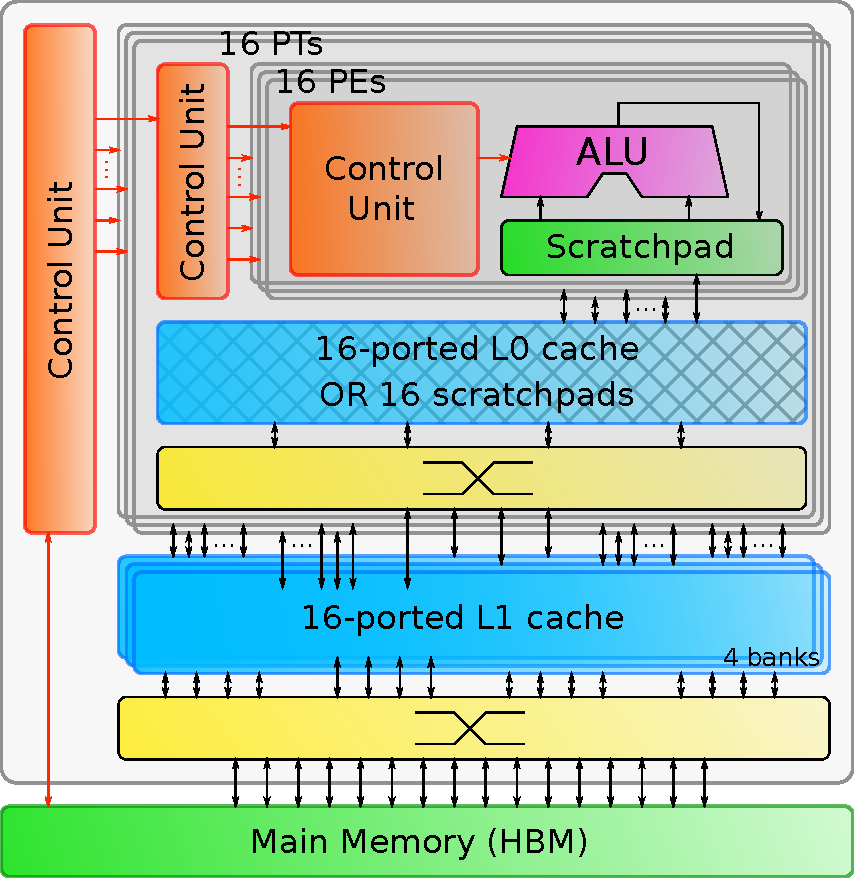
\includegraphics[width=0.7\textwidth]{Chapter_SoA/Figures/PDF/OuterSPACE.pdf}
            \caption{Architecture of OuterSPACE}
            \label{fig:soa:outerspace}
        \end{figure}
    \end{minipage}
    \hfill
    \begin{minipage}[b]{0.49\linewidth}
        \begin{figure}[H]
            \centering
            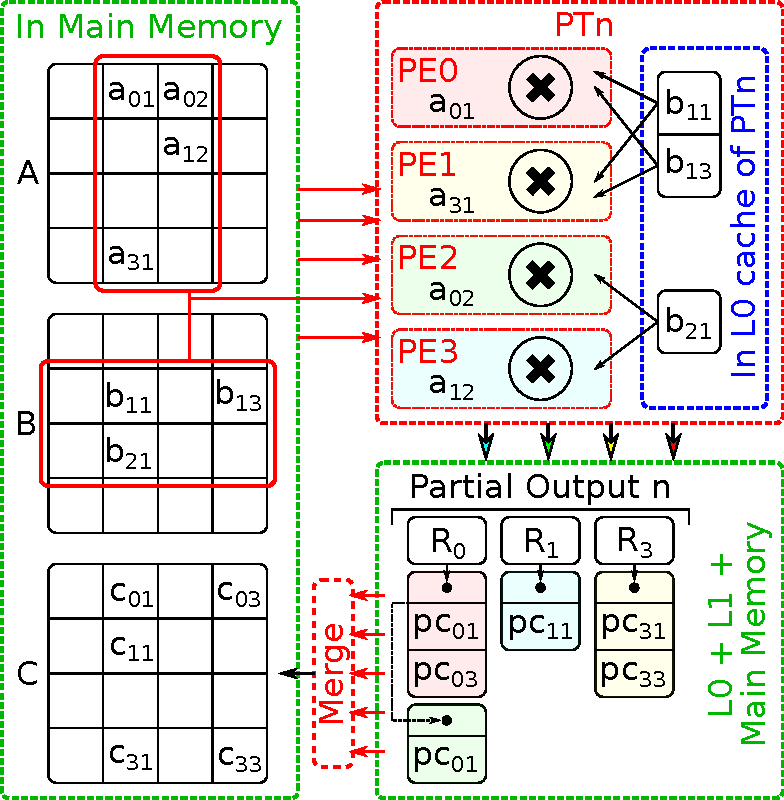
\includegraphics[width=0.705\textwidth]{Chapter_SoA/Figures/PDF/OuterSPACE_How_Vertical.pdf}
            \caption{OuterSPACE Data Flow}
            \label{fig:soa:outerspaceHow}
        \end{figure}
    \end{minipage}
\end{figure}

% %%%%%%%%%%%%%%%%%%%%%%%%%%%%%%%%%%%%%%%%%%%%%%%%%%%%%%%%%%%%%%%%%%%%%
% %% State-of-the-Art %%
% ExTensor
% %%%%%%%%%%%%%%%%%%%%%%%%%%%%%%%%%%%%%%%%%%%%%%%%%%%%%%%%%%%%%%%%%%%%%

\subsection{ExTensor}
\label{sec:soa:extensor}

The authors created ExTensor~\cite{Hegde2019_ExTensor} as a general purpose sparse tensor algebra accelerator (including SpMSpM). It is an \algo{OP} accelerator but due to its support for three levels of fixed \emph{tiling} of the inputs, it optimizes the \emph{intersection} search between non-zero elements or \emph{tiles}\footnote{Tensauraus~\cite{Srivastava2020_Tensaurus} is another accelerator designed for tensors, but their focus is on SpMM.}. By doing the \emph{intersections} ahead of time, at different levels of the memory hierarchy (which correspond to the \emph{tile} levels), ExTensor is able to efficiently eliminate \emph{ineffectual operations}, thus addressing the main issue in \algo{IP} or complex \emph{tiling} algorithms. Indeed, the input matrices would typically be stored in an \emph{(UOP, UOP, UOP, CP}) format, corresponding to three levels of \emph{tiling}.
ExTensor is designed with a flexible architecture composed of different bricks (see Figure~\ref{fig:soa:extensor}). To simply aid in the understanding, the interactions between the bricks are described using function calls:
\begin{itemize}
    \item The \emph{Scanner} is a storage unit that delivers a stream of coordinates in increasing order, fetching them from memory. The coordinates are delivered through the \emph{Iterate()} operation call.
    \item The \emph{Intersect} is a hardware block that co-iterates over several \emph{Scanners} in parallel and compares the coordinate streams. This unit performs the \emph{intersection} search required by \algo{IP} type algorithms, delivering a single stream with the matching coordinates, which are the coordinates of non-zero \emph{partial sums}. To optimise the \emph{intersection} step, it is possible to skip a range of coordinates in a stream depending on the current coordinate of another stream. Thus, the \emph{Intersect} sends skip messages with \emph{SkipTo()} operations to the other \emph{Scanners}.
    \item The \emph{Coordinator} is a hardware unit that includes \emph{Scanners} and \emph{Intersect} units, and manages the input and output data depending on the current processed \emph{tile}, as shown in Figure~\ref{fig:soa:extensor}. Data and \emph{metadata} are respectively stored in storage units and \emph{Scanners}, while a \emph{Sequencer} manages the \emph{Iterate()} calls so that the \emph{Intersect} brick delivers the stream of effective coordinates. In addition, in the \emph{Tile Coord} brick, the offsets of the \emph{tile} are added back, so the output of the \emph{Coordinator} is in absolute coordinates.
\end{itemize}

These bricks can be placed at different positions in a memory hierarchy, depending on the \emph{tiling} and selected hardware. Thus, the \emph{Coordinator} is able to intersect at coarse-granularity with output data being \emph{metadata} of the next \emph{tile}, skipping an entire \emph{tile} when appropriate, with low computation cost, and also at fine-granularity when output data are the non-zero elements that need to be multiplied.

ExTensor is designed with three levels of \emph{tiling} that each have  either input or output sequentiality. First, a \emph{Sequencer} plus \emph{Scanners} block~\ding{192} is placed close to the main memory to determine which \emph{tiles} to send to the next storage, the \emph{Last Level Buffer} (\emph{LLB}). Then, for each \emph{tile}, a \emph{Coordinator}~\ding{193} in the \emph{LLB} intersects the next level \emph{tiles}, which are sent to several \emph{PEs} that will process in parallel. Finally, in each \emph{PE}, a \emph{Coordinator}~\ding{194} intersects the non-zero elements of the computed \emph{tile} and sends them to the arithmetic unit of the \emph{PE} for multiplication.

In addition to these bricks which are the main contributions, ExTensor still needs to perform the \emph{merge} phase, including the \emph{reduction} of the \emph{POs} which are stored in \emph{CP$^{2}$} format. The \emph{Partial Output Buffer} (\emph{POB}), is managed by \emph{tiles}, and the content of the \emph{tile} is stored on-chip using a Content Addressable Memory (CAM) for quick access, enabling \emph{reductions} to be performed. On overflow, the \emph{tiles} are flushed to main memory. To benefit from ExTensor's support for \emph{tiling}, the input matrices need preprocessing, making it difficult to directly compare performance with other accelerators.

\begin{figure}
    \centering
    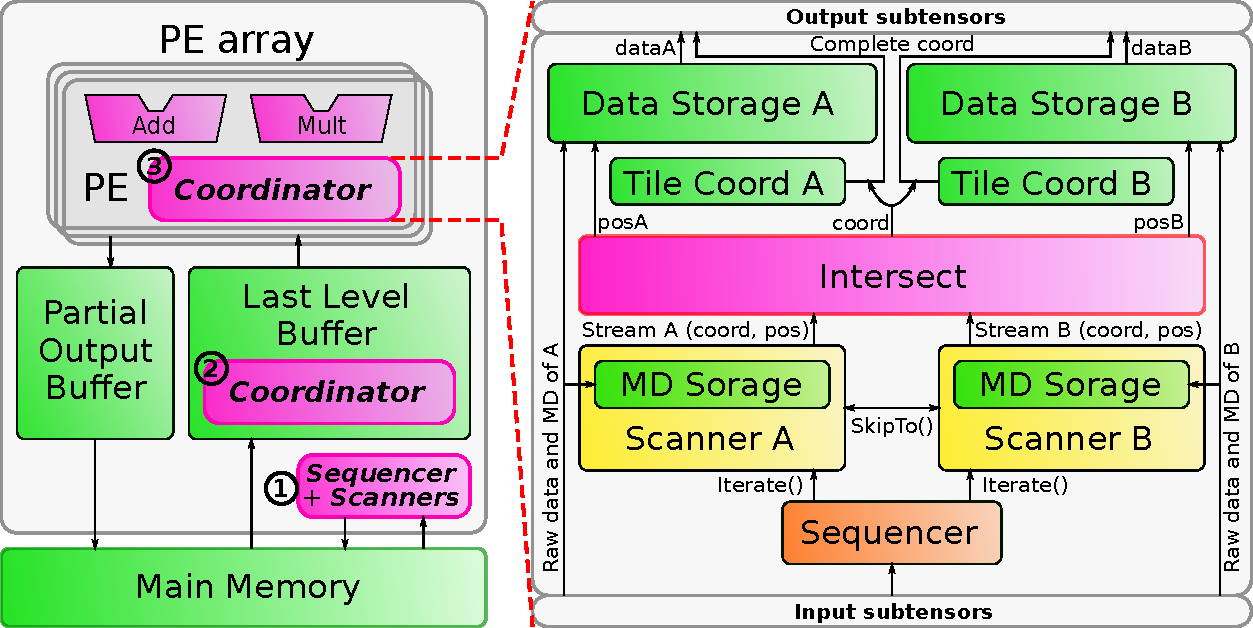
\includegraphics[width=0.6\linewidth]{Chapter_SoA/Figures/PDF/ExTensor.pdf}
    \caption{Architecture of ExTensor}
    \label{fig:soa:extensor}
\end{figure}

% %%%%%%%%%%%%%%%%%%%%%%%%%%%%%%%%%%%%%%%%%%%%%%%%%%%%%%%%%%%%%%%%%%%%%
% %% State-of-the-Art %%
% Gamma
% %%%%%%%%%%%%%%%%%%%%%%%%%%%%%%%%%%%%%%%%%%%%%%%%%%%%%%%%%%%%%%%%%%%%%

\subsection{Gamma}
\label{sec:soa:gamma}

Gamma~\cite{Zhang2021_Gamma} is a dedicated accelerator for SpMSpM kernels, which uses \algo{Gust} algorithm. The two input matrices are both stored in \emph{(UOP, CP) row-major} format and the output is generated in the same format, providing consistency.

% Figure in Accelerators.tex

The Gamma architecture, presented in Figure~\ref{fig:soa:gamma}, is composed of a fetcher for the $A$-rows that contains a \emph{Distributor} to distribute them to 32 \emph{PEs}. Each \emph{PE} processes an entire $A$-row and computes the corresponding $C$-row. The \emph{PE} fetches the required $B$-rows and merges and sorts them in a 64-wide \emph{merge} block, before multiplying with the $A$-elements. As a result, the output $C$-row  is generated in order. The \emph{reduction} step is, thus, highly simplified, because any duplicate indices are adjacent. Normally, the $C$-row can be written back to main memory. However, if the $A$-row contains more than 64 non-zero elements, then it must be processed with multiple passes. After each pass, the partial $C$-row is stored temporarily. Finally, the temporary $C$-rows are read-back and merged by the \emph{PEs}.
Of course, the $B$-rows must be accessed repeatedly by the different \emph{PEs}, and Gamma proposes \emph{FiberCache} which is a highly banked cache which fetches the $B$-rows in advance, based on the column index table of $A$. It keeps track of which rows of $B$ are most needed by the \emph{PEs}, and when an eviction is necessary, the victim, is the row which is least needed.

Gamma encounters some difficulties when the $A$-matrix has rows that are too dense, requiring multiple iterations through the \emph{PEs}, which creates a high-load on the cache. The authors propose a software preprocessing technique which splits dense $A$-rows and rearranges them to make best use of the \emph{FiberCache}.

% %%%%%%%%%%%%%%%%%%%%%%%%%%%%%%%%%%%%%%%%%%%%%%%%%%%%%%%%%%%%%%%%%%%%%
% %% State-of-the-Art %%
% PHI
% %%%%%%%%%%%%%%%%%%%%%%%%%%%%%%%%%%%%%%%%%%%%%%%%%%%%%%%%%%%%%%%%%%%%%

\subsection{PHI}
\label{sec:soa:phi}

The authors of PHI~\cite{Mukkara2019_PHI} focus on graph algorithms, and include the \acrshort{spmv} kernel as it is core in graph processing.
They note that many large graph algorithms favour pull implementations (each node reads inputs from its neighbours) compared to push implementations (each node propagates results to its neighbours), since in a traditional memory system, push implementations require read-modify-writes which require accessing complete cache-lines, even though a small unit of data is modified.
The push implementation corresponds to the \acrshort{op} algorithm, which suffers from poor memory performance with traditional caches.

PHI is essentially a modified cache which is optimized to efficiently process commutative\footnote{As PHI focuses on graph algorithms, the \gls{reduction} operation could be any commutative operator including logical operations (OR/AND) as well as addition.} \gls{scatter} updates, also called \glspl{reduction}.
It stores, and coalesces values to update, in the cache, as shown in Figures~\ref{fig:soa:phi} and~\ref{fig:soa:phiHow}.
This type of cache is called a \gls{redC}.
PHI works in two phases, managing to take advantage of the two version of the \acrshort{op} algorithm: \textit{immediate updates} and \textit{deferred updates}.
Three new features are introduced, compared to a standard cache:
\begin{itemize}
    \item \textit{In-cache \gls{reduction} storage and processing}.
    In the first phase, when an update for a line not in the cache is received (cache-\gls{miss}), the cache does not fetch the data-line from memory, but rather marks a free cache-line as being in \textit{buffer mode} (\textit{B}), and simply locally stores the update.
    If there are subsequent updates that \gls{hit} the cache-line, they are stored, or combined, using the in-cache commutative operator, as shown in the case~1 of Figure~\ref{fig:soa:phiHow} (top).
    When a cache-line is evicted, if it contains multiple updates, PHI assumes that the coalescing has been effective, and it updates the main memory via a line-wise read-accumulate-write operation.
    This is the normal mode of operation of a traditional \gls{redC}, which processes \textit{immediate updates}.
    %
    \item \textit{Output Batching}.
    In the first phase, if a cache-line is evicted, but contains few updates (managed with a configurable threshold), PHI batches these updates as \textit{(address, value)} tuples, allocating a new cache-line in \textit{update batching mode} (\textit{UB}) to assemble the batch, as shown in the case~2 of Figure~\ref{fig:soa:phiHow} (bottom).
    Groups of updates are organized by \textit{bins} corresponding to a small memory region.
    The batches are streamed to main memory, assembling the \acrfullpl{po} typical of the \textit{deferred updates} \acrshort{op} version.
    Later, in the second phase, the \textit{deferred updates} are read back and processed.
    The reading of the batches is efficient, as they are contiguous (see the \acrshort{op} algorithm in Section~\ref{sec:bg:algos}).
    %
    \item \textit{Reduced Cache Synchronization Traffic}.
    When scaling PHI to multi-core systems, private caches act as local buffers, coalescing the updates and reducing coherency protocol traffic.
\end{itemize}

\begin{figure}[htbp]
    \centering
    \begin{minipage}[b]{0.44545455\linewidth}
        \begin{figure}[H]
            \centering
            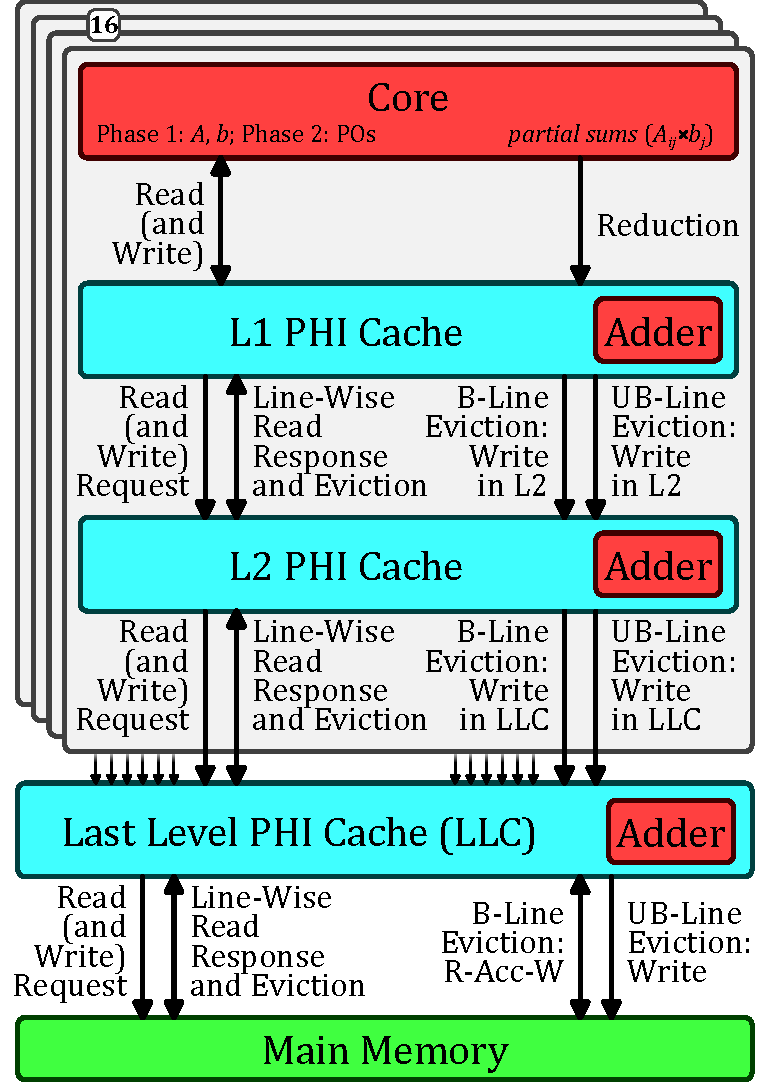
\includegraphics[width=\linewidth]{Chapter_SoA/Figures/PDF/SoA_AcceleratorsArchis_PHI.pdf}
            \caption{Architecture of PHI}
            \label{fig:soa:phi}
        \end{figure}
    \end{minipage}
    \hfill
    \begin{minipage}[b]{0.53636364\linewidth}
        \begin{figure}[H]
            \centering
            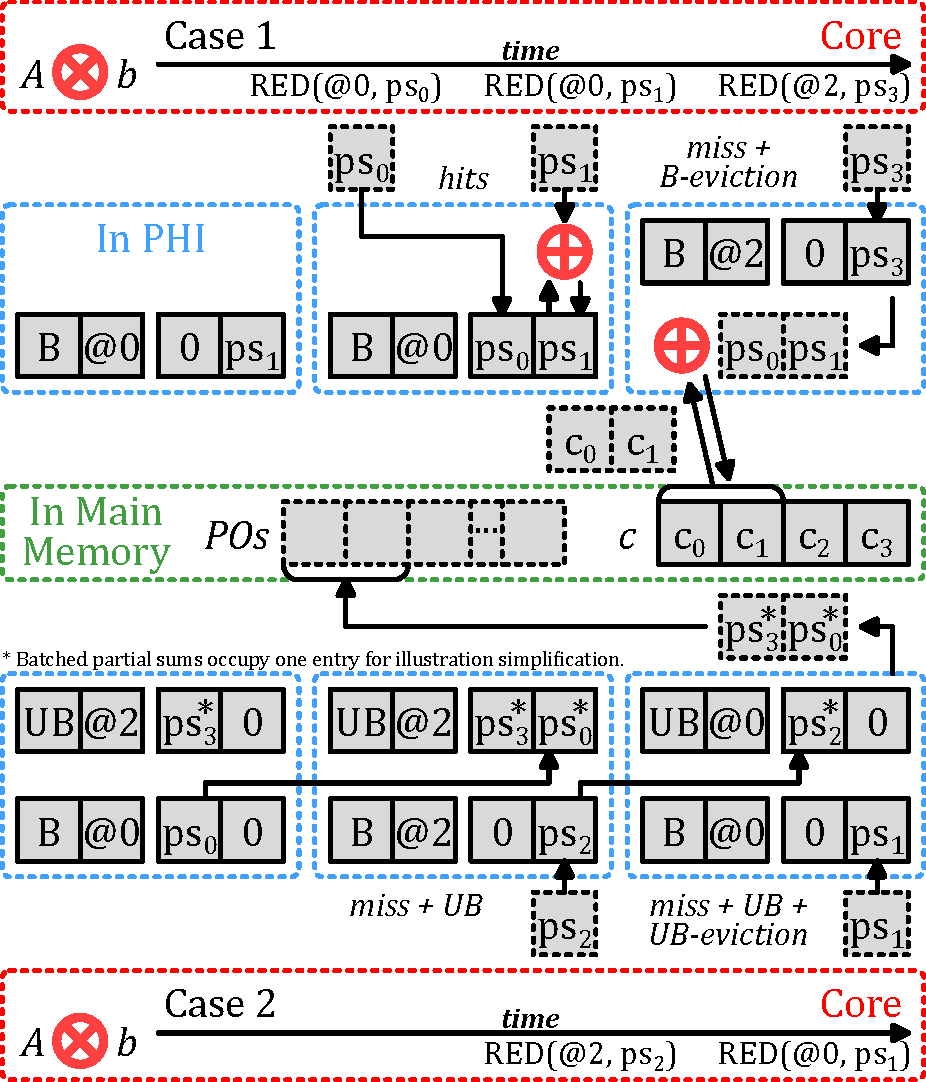
\includegraphics[width=\linewidth]{Chapter_SoA/Figures/PDF/SoA_AcceleratorsArchis_PHI_DF.pdf}
            \caption{PHI Dataflow}
            \label{fig:soa:phiHow}
        \end{figure}
    \end{minipage}
\end{figure}

This combination of in-cache coalescing and update buffering enables PHI to take advantage of locality when possible (like Coup~\cite{Zhang2015_Coup}), but with the addition of \textit{UB}, PHI improves memory utilization, even when the data being updated is too large to fit in the cache.
For \acrshort{spmv}, the authors report that much of the benefit comes from the \gls{reduction} in memory synchronization traffic for multi-core systems.

\begin{highlight}{Conclusion}{Red}
    \textbf{PHI} is a \gls{reduction}-aware cache architecture that optimizes commutative \gls{scatter} updates by combining in-cache coalescing, output batching, and reduced synchronization traffic, effectively improving memory utilization for both \textit{immediate} and \textit{deferred update} \acrshort{op} \acrshort{spmv} kernel.
\end{highlight}

% %%%%%%%%%%%%%%%%%%%%%%%%%%%%%%%%%%%%%%%%%%%%%%%%%%%%%%%%%%%%%%%%%%%%%
% Other Accelerators
% %%%%%%%%%%%%%%%%%%%%%%%%%%%%%%%%%%%%%%%%%%%%%%%%%%%%%%%%%%%%%%%%%%%%%
\subsection{Other Accelerators}
\label{sec:soa:other_accel}

In the above sections, we have described four sparse accelerators, covering different matrix multiplication algorithms and architectures.
In the following paragraphs we present the other accelerators which we cover in less detail, to expose the reader to the diversity of architectures.

\ref{app:other_acc}


\bigskip\bigskip

Coup cache coherence protocol
PHI
SortCache
SpDCache (merger and are is high)
ASA (additional cache, mm)

C3ache (GPGPU, mm, op-Gust)

+ reductions in cache, scatter, general purpose, scalable, minor area overhead
- compute is deferred (potential bottleneck)

SPiDRE
SSSR (riscv)
ExTensor *
simple, main memory or core, gather, streaming and intersection, general purpose
Spider heavy compared to in cache/core solutions, traffic on main mem
SSSR light weight, but necessitate in core integration
ASA is near core only, easier





EIE
SDMA (adaptative gust, hw/sw)
SCNN SparTen CANDLES SparTA MaxK-GNN
DNN ASIC weight and activation sparsity
Funnel (mm)
prediction based
FullSparse
mm, dense and sparse mode, detector


GraphR (graph, spmv)
SpaceA (spmv)
GAS (general purpose)
In memory
great potential for data reuse and low traffic
but Apparoches based on analog compute in memory can only work with low precision data and are not applicable for HPC.


SDE
SPAGHETTI (MM, op)
Sextans (mm)
MOSCON (op, mm, dnn)
GSCSp (mm, gust)
DySpMM (mm)
Leda (mm, gmm, op)
AiSpGEMM
highly tuned for an FPGA implementation (some HBM equipped)
HBM optimized HiSparse
Graph specific HitGraph GraphLily ThunderGP



ITS (graph, spmv)
SPU (general purpose -> sparse and dense applications)
Alrescha (configurable -> general purpose, but IP only)
InnerSP (gust)
Mentor (gust)
ScanNow (mm, gust inspired)
High perf, because avoid synchronization bottlenecks and minimize memory on chip traffic, but high area overhead
Scalability is delicate (big mergers and lookup tables)

Tensaurus
Tensors -> general purpose, highly tiled
Depend on specific sparse storage
not HARP
Block-SpMM vectorSparse Flash-LLM TC-GNN DTC-SpMM

MatRaptor (gust, special format)
SpArch (domain specific, op -> POs)
SIGMA (ip, DNN)
RTSpMSpM (application specific)
Focus on MM

CoSPARSE (spmv, hw/sw)
Spada (hw/sw, mm, adaptative)
Flexagon (mm, dnn)
ACES (gust based, mm)
Sparm (mm)
Vesper (general purpose)
IOPS (mm)
DMSA (gust based, mm)
Multi algo, adapt to the matrix structure, more general purpose
more delicate on scalability -> do everything is costly

SPADES
gzip decompression

\begin{highlight}{Conclusion}{Red}
    This comprehensive overview demonstrates that sparse matrix accelerators have evolved significantly from \textbf{2015 to 2025}, with diverse architectural approaches addressing different algorithmic paradigms, memory hierarchies, and sparsity patterns to maximize performance and energy efficiency when handling increasingly irregular and diverse sparse workloads in machine learning, graph processing, and scientific computing.
\end{highlight}